\documentclass[twoside,11pt]{article}\usepackage{amsmath,amsfonts,amsthm,fullpage}
\usepackage{amsmath}
\usepackage{amssymb}
\usepackage{listings}
\setlength{\parindent}{0pt}
\usepackage{graphicx}
\usepackage{bm}
% Use the standard article template.
%
% The geometry package allows for easy page formatting.
\usepackage{geometry}
\geometry{letterpaper}
% Load up special logo commands.
\usepackage{doc}
% Package for formatting URLs.
\usepackage{url}
% Packages and definitions for graphics files.
\usepackage{epstopdf}
\DeclareGraphicsRule{.tif}{png}{.png}{`convert #1 `dirname #1`/`basename #1 .tif`.png}

\def\argmin{\operatornamewithlimits{arg\, min}}
\newcommand{\rbr}[1]{\left(#1\right)}
\newcommand{\cbr}[1]{\left\{#1\right\}}
\newcommand{\Ncal}{\mathcal{N}}

%
% Set the title, author, and date.
%
\title{
Parallel Algorithm - Solve system of linear equations with Jacobi method with MPI
}
\author{
  D'Souza, Ajay\\
  \texttt{ajaydsouza@gatech.edu}
}
\date{\today}

\begin{document}


\maketitle



% Add an abstract.
\begin{abstract}
Implement Parallel Algorithm to solve a system of linear equations us the Jacobi method
\end{abstract}

% Add various lists on new pages.
\pagebreak
\tableofcontents

\pagebreak
\listoffigures


% Start the paper on a new page.
\pagebreak

%
% Body text.
%
\section{Algorithm Description}
\label{algorithm}
\begin{enumerate}
\item
We are given a square matrix of size $n$ and $p$ the available processors where $p$ is a perfect square. We will embed a logical square matrix of size  $\sqrt{p}\times\sqrt{p}$ on to the hypercubic processors $p$ using $\verb|MPI_Cart_Create|$. 
\item
A property of this embedding is that the processors in a row or a column of the logical $\sqrt{p}\times\sqrt{p}$ matrix are hypercubic connected processors
\item
The $(0,0)$ processor or the rank $0$ processors reads the input matrix A,b and has to block distribute it to the other relevant processors
\item
The processors in the first column of the matrix have to get the vector $b$ block distributed to them from the rank $0$ processor in that column. This can be done by a $\verb|MPI_Scatterv|$ along the first column with the count and displacement arrays set to the appropriate $\lceil \frac{n}{\sqrt{p}} \rceil$ or $\lfloor \frac{n}{\sqrt{p}} \rfloor$ offset and count depending on if the rank of the processor is $< (n \mod \sqrt{p})$  or not. The complexity of this operation is $ \mathcal{O}(\tau \log \sqrt{p} + \mu n)$
\item
Next we have to distribute the $n\times n$ matrix A from processor of rank $0$ to every processor in the matrix so each processor has a local A block matrix of size $\frac{n}{\sqrt{p}} \times \frac{n}{\sqrt{p}}$. 
\item
This is implemented using $\verb|MPI_Scatterv|$. The count and displacement arrays let us provide varying size of rows and columns that need to be block distributed to a processor based on its rank and of $n$ not being a multiple of $\sqrt{p}$. Matrix A is stored as an one dimensional array and non contiguous elements from the array would need to be scattered. This can be accomplished with creating a $\verb|MPI_Type_vector|$ which takes as input a count,block length and stride
\item
Since this involved scattering the elements along column and then along rows of processors which are hypercubic the run time complexity is
\begin{align}
&= \mathcal{O}(\tau \log \sqrt{p} + \mu n^2) + \mathcal{O}(\tau \log \sqrt{p} + \mu \frac{n^2}{\sqrt{p}})\nonumber\\
&= \mathcal{O}(\tau \log \sqrt{p} + \mu n^2) \label{l_1}
\end{align}
\item
Once the processors in the first column receive the block distributed rows of matrix A, those processors can keep an array local $local_D$ of $\frac{n}{\sqrt{p}}$ elements from the block distributed $local_A$, which correspond to the diagonal elements of the $n\times n$ matrix A.
\item
Or these diagonal elements of the $n\times n$ matrix A, could also be got by the processors in the first column, from the local block matrix A $local_A$ in the diagonal processors in the row of each column $(i,i)$. The sending and receiving can be performed by $\verb|MPI_Send|$ and $\verb|MPI_Recv|$ for a complexity of $\mathcal{O}(1)$
\item
Finally to perform the matrix multiplication $Ax$, each processor in column $i$ would need to have the bock distributed $local_x$ vector of size $\frac{n}{\sqrt{p}}$ from the $i^{th}$ processor in the first column
\item
This transpose broadcast of local $x$ can be performed using the following steps
\begin{enumerate}
\item
Each $i{th}$ processor in the left column will send its local $local_x$ array of size $\frac{n}{\sqrt{p}}$ to the diagonal processor ($i,i)$ in that row using $\verb|MPI_Send|$ and $\verb|MPI_Recv|$, this is of complexity $\mathcal{O}(1)$
\item
The diagonal processor $(i,i)$ in every row will then broadcast these $\frac{n}{\sqrt{p}}$ local $local_x$ elements to each processor in its column using $\verb|MPI_Bcast|$, this is of complexity $\mathcal{O}(\tau+\mu \frac{n}{\sqrt{p}}) \log \sqrt{p}$
\end{enumerate}
\item
Now each processor in the processor matrix of size $\sqrt{p}\times \sqrt{p}$ has a block allocated local A matrix $local_A$ and a local x vector $local_x$ and can perform a matrix vector multiplication
\item
Matrix multiplication is performed in each processor with a complexity of $\mathcal{O}({(\frac{n}{\sqrt{p}})}^2)$
\item
The multiplication results in a local y $local_y$ vector of size  $\frac{n}{\sqrt{p}}$ on each processor. 
\item
Now the corresponding elements of local y, in every processor in a row are added and stored in the local $y$ vector of size $\frac{n}{\sqrt{p}}$ of the processor in the first column in each row using. This operation can be performed with $\verb|MPI_Reduce|$ with a complexity of $\mathcal{O}(\tau  + \mu \frac{n}{\sqrt{p}} ) \log \sqrt{p}$
\item
The processors in the first column now have the local $local_y$,$local_D$ and $local_b$ arrays of size $\frac{n}{\sqrt{p}}$. Then can now compute the the new x as $x_i = \frac{(local_{b_i} - (local{y_i} -local_{D_i}*local_{x_i}))}{local_{D_i}}$
\item
The new x computed in the processors in the first column in each row is stored in the $local_x$ vector on that processor
\item
Now this new $local_x$ is transpose distributed back from the $i^{th}$ processor in the first row to the processors in the $i^{th}$ column using transpose broadcast as described earlier
\item
With the new $\frac{n}{\sqrt{p}}$ local $local_x$ values at each processor will perform another matrix multiplication $local\_y= local\_A local_x$ as described above.
\item
The results from local y from the processors in a row are summed up back to the first processors in that row as described earlier
\item
Each processor in the first column can then compute the 2 norm of $|local_b-local_y|$
\item
We can then do a $\verb|MPI_AllReduce|$ to sum the local 2 norm of all processors in the grid to get the 2 norm of $|b-AX_{new}|$. The value of the 2 norm for the whole matrix will now be available on each processor in the matrix. 
\item
This way every processor can check if the 2 norm is within the tolerance specified and exit the loop in the same way as other processors. This step of computing the norm using  $\verb|MPI_AllReduce|$ should be of complexity 
\begin{align}
&= \mathcal{O}(\tau+\mu)\log \sqrt{p} + \mathcal{O}(\tau+\mu)\log \sqrt{p}\nonumber\\
&= \mathcal{O}(\tau+\mu)\log \sqrt{p} \label{l_2}
\end{align}
\item
If the 2 norm of $b-AX_{new}$ is beyond the tolerance specified and if we have still not reached the cut off iteration then each processor will continue the iteration
\item
On continuing the iteration the first column processors already have the value of the new $local_y$ from the last $AX_{new}$.So the first column processors can compute the new $local_{x_{new}}$ and then transpose broadcast it as described earlier and continue till convergence
\item
On termination of the iteration, only the processors in the first column need to send their $local_x$ values to the rank $0$ processor. This can be done using $\verb|MPI_Gather|$. This takes $\log \sqrt{p}$ steps and since we start by sending message of size $\frac{n}{\sqrt{p}}$ till we reach $\frac{n}{2}$. So the complexity of this operation will be $\mathcal{O}(\tau \log \sqrt{p} + \mu n)$
\end{enumerate}






\pagebreak
\section{Performance Plots}
The algorithm was executed for the following parameters
\begin{itemize}
\item
size n = 500,1000,2000,4000,8000,10000,12000,14000,16000,16000,20000,25000
\item
Difficulty d = 0.5,0.75,0.9,0.95
\item
Number of parallel processors p=4,9,16,25
\end{itemize}


\subsection{Runtime Performance Plots}

The following are the Run Time plots

\subsubsection{Runtime Performance for Serial Algorithm P=1}

\begin{figure}[!htbp]
\centering
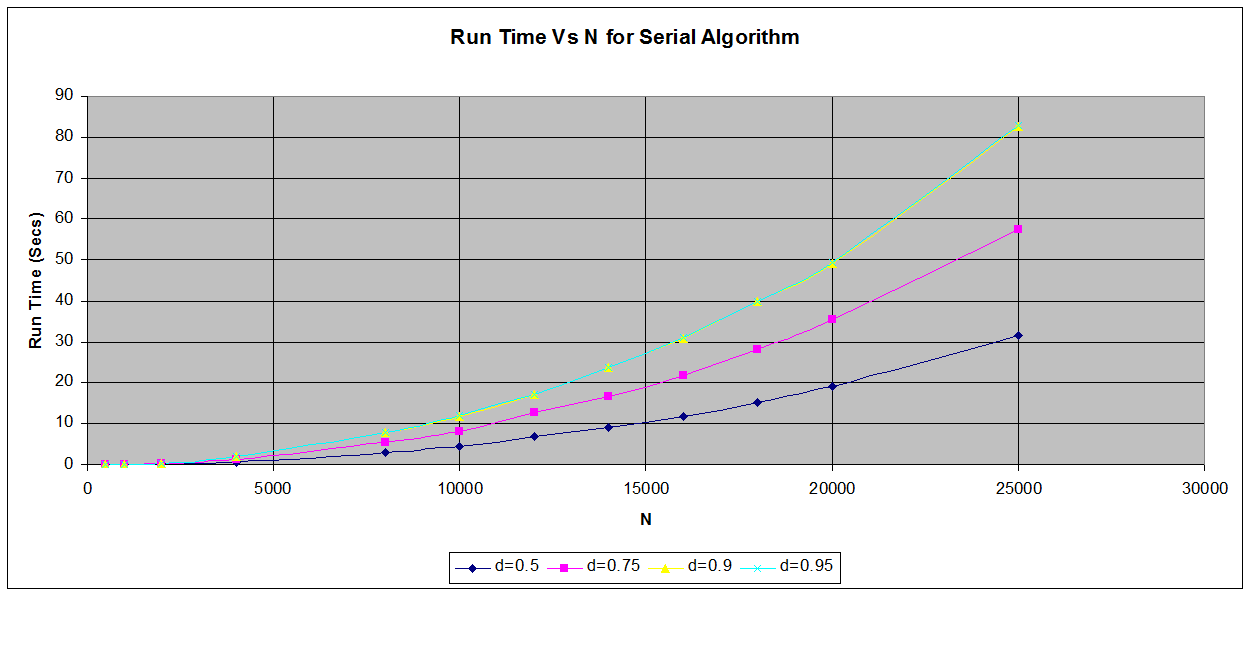
\includegraphics[scale=.46]{charts/runtime_n_d_p_1_serial} 
\caption{Serial Runtime Vs N}
\label{Serial Runtime Vs N}
\end{figure}



\pagebreak
\subsubsection{Runtime Performance - Plot of Run Time Vs N for different levels of difficulty for fixed No of Processors P}
The following is the performance plot of Runtime Vs N the matrix dimension for different levels of difficulty for a fixed number of processors.

\begin{enumerate}
\item
P=4 $\eqref{Run Time Vs N for P=4}$
\item
P=9 $\eqref{Run Time Vs N for P=9}$
\item
P=16 $\eqref{Run Time Vs N for P=16}$
\item
P=25 $\eqref{Run Time Vs N for P==25}$
\end{enumerate}

\begin{figure}[!htbp]
\centering
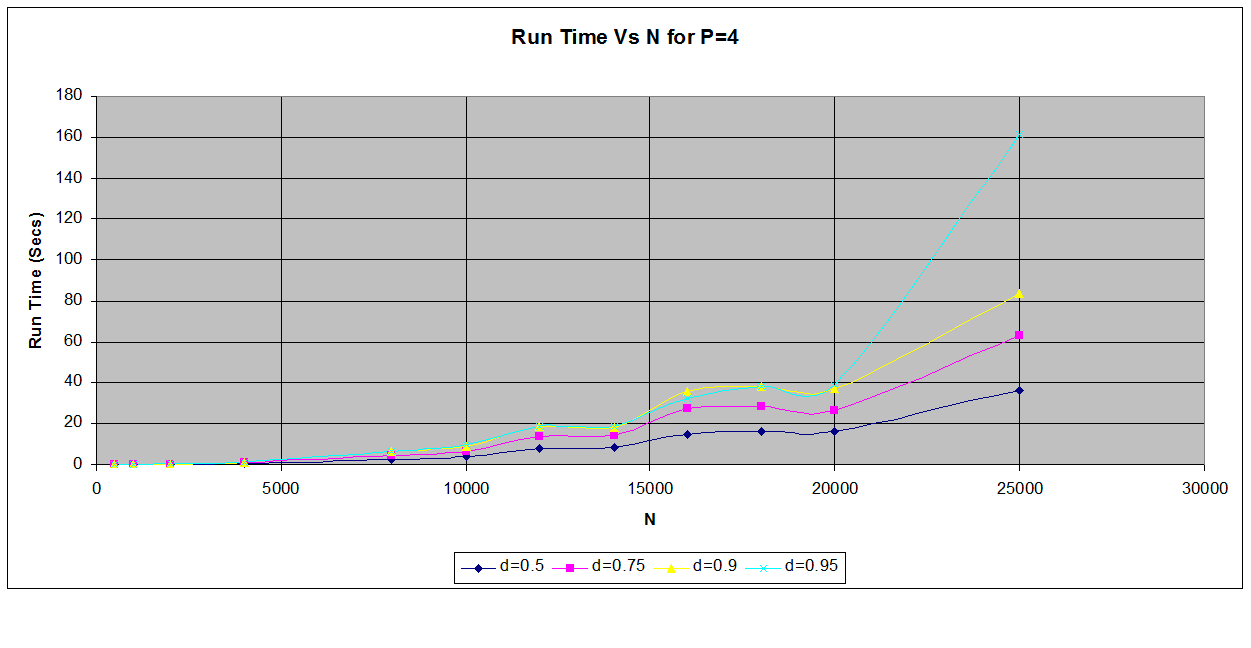
\includegraphics[scale=.46]{charts/runtime_n_d_p_4} 
\caption{Run Time Vs N for P=4}
\label{Run Time Vs N for P=4}
\end{figure}

\begin{figure}[!htbp]
\centering
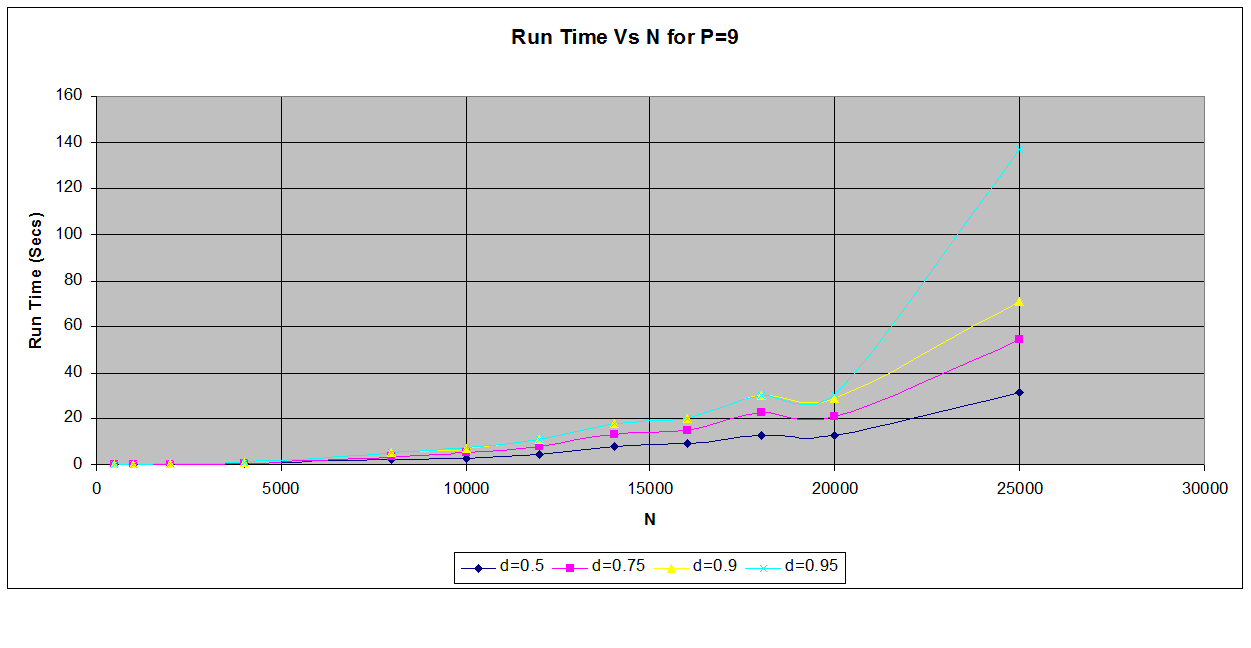
\includegraphics[scale=.46]{charts/runtime_n_d_p_9} 
\caption{Run Time Vs N for P=9}
\label{Run Time Vs N for P=9}
\end{figure}

\begin{figure}[!htbp]
\centering
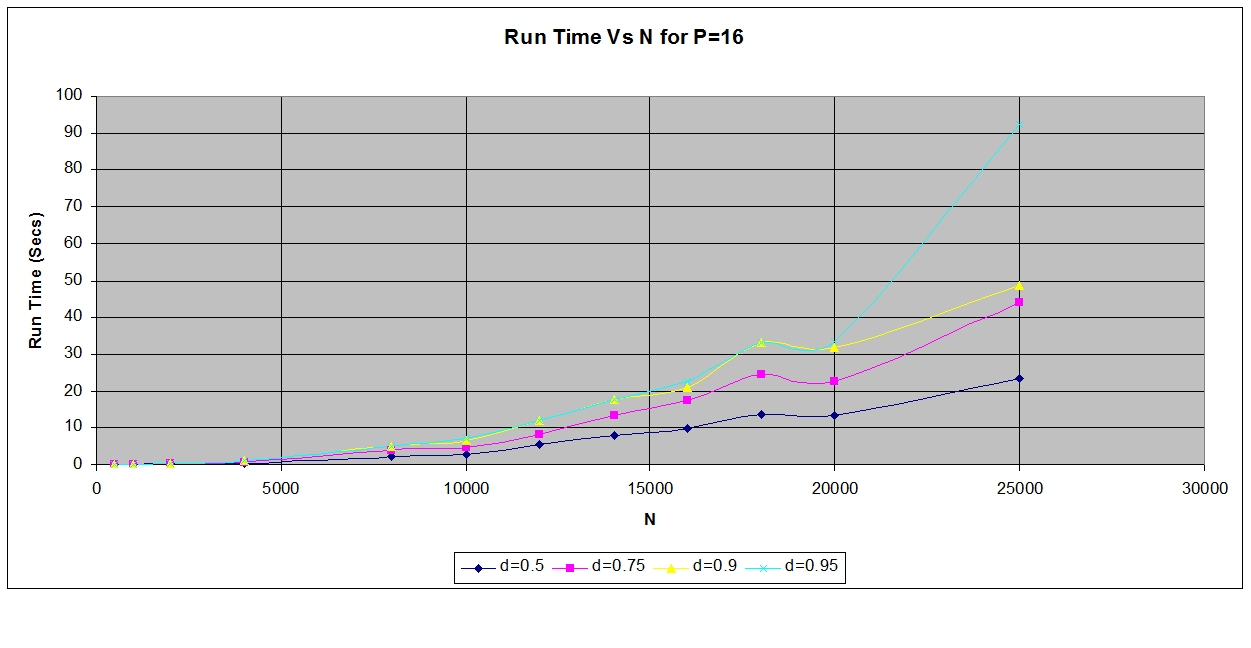
\includegraphics[scale=.46]{charts/runtime_n_d_p_16} 
\caption{Run Time Vs N for P=16}
\label{Run Time Vs N for P=16}
\end{figure}

\begin{figure}[!htbp]
\centering
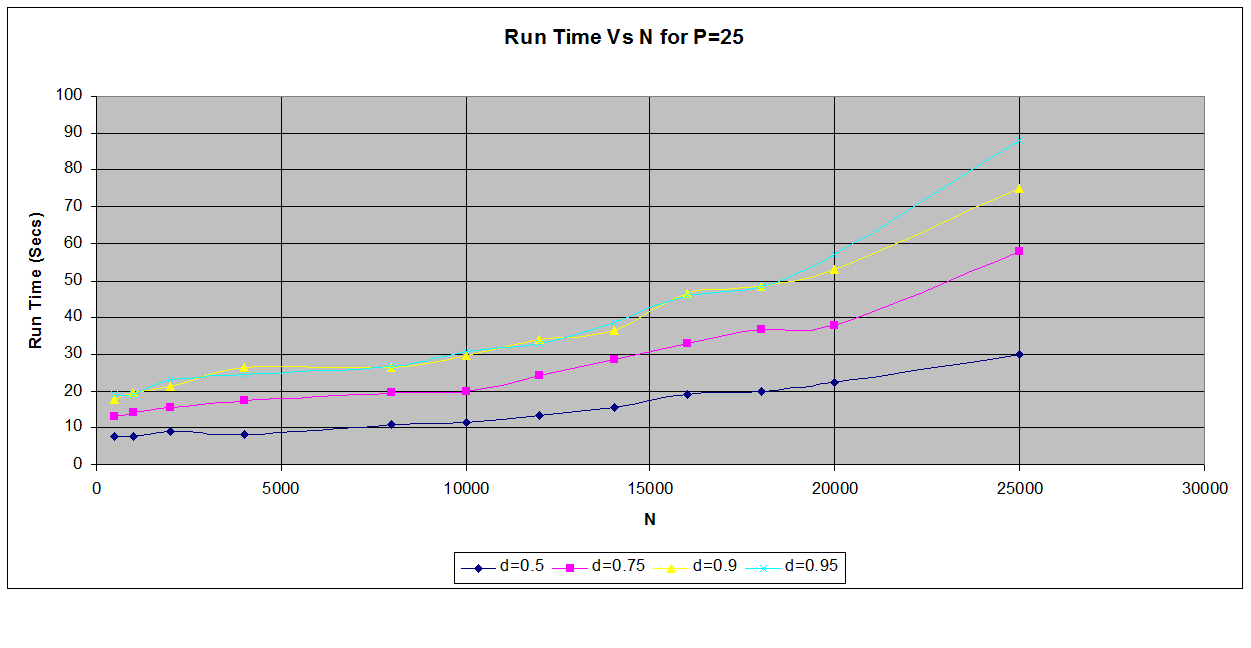
\includegraphics[scale=.46]{charts/runtime_n_d_p_25} 
\caption{Run Time Vs N for P==25}
\label{Run Time Vs N for P==25}
\end{figure}



\pagebreak
\subsubsection{Runtime Performance - Plot of Run Time Vs Number of Processors P for different levels of difficulty for fixed size N}
The following is the performance plot of Run Time Vs Number of Processors P for different levels of difficulty for fixed matrix size N

\begin{enumerate}
\item
N=1000 $\eqref{Run Time Vs P for N=1000}$
\item
N=8000 $\eqref{Run Time Vs P for N=8000}$
\item
N=16000 $\eqref{Run Time Vs P for N=16000}$
\item
N=20000 $\eqref{Run Time Vs P for N=20000}$
\item
N=25000 $\eqref{Run Time Vs P for N=25000}$
\end{enumerate}

\begin{figure}[!htbp]
\centering
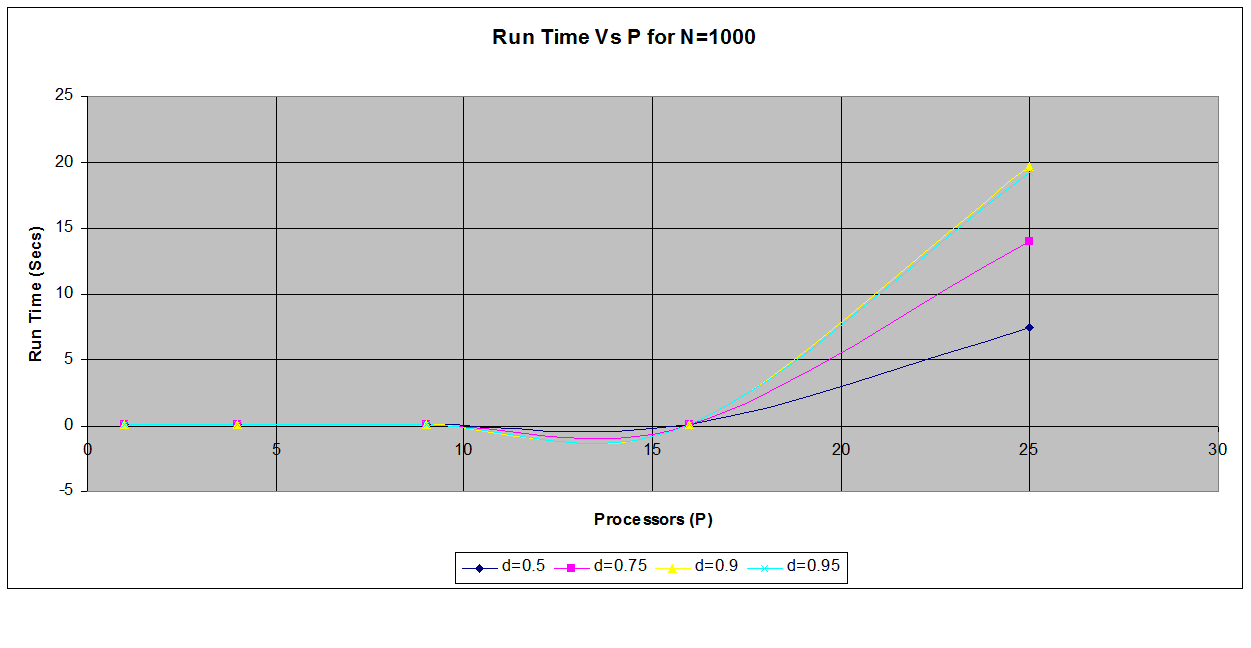
\includegraphics[scale=.46]{charts/runtime_p_d_n_1000} 
\caption{Run Time Vs P for N=1000}
\label{Run Time Vs P for N=1000}
\end{figure}

\begin{figure}[!htbp]
\centering
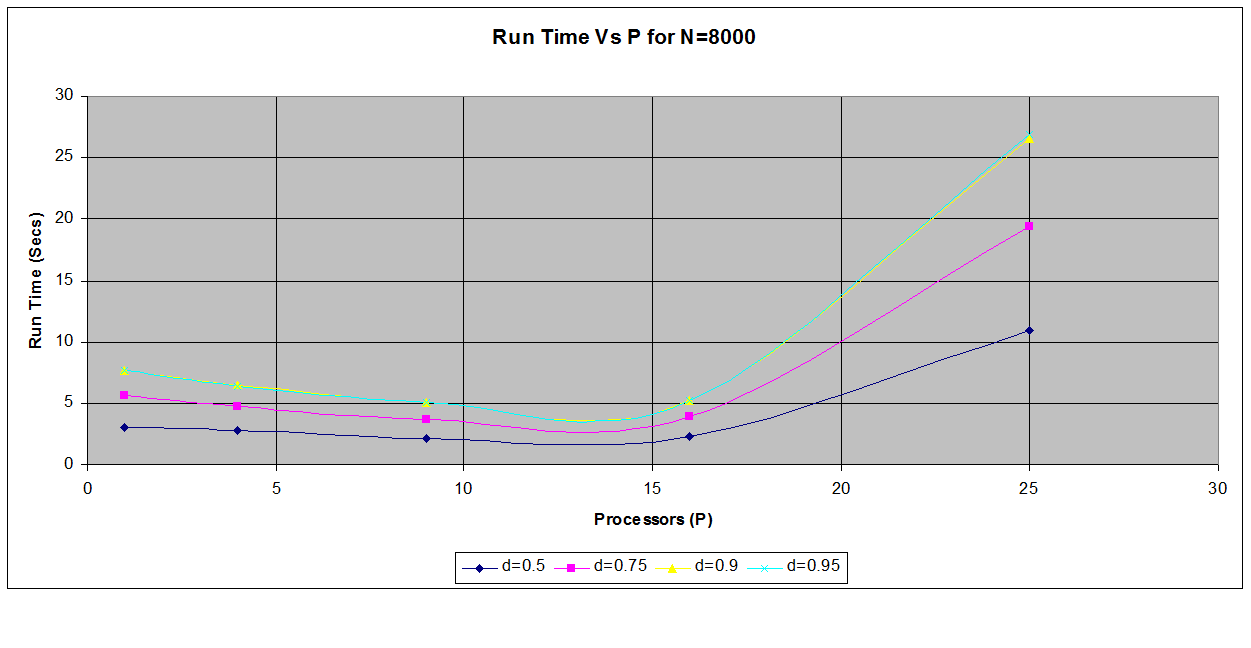
\includegraphics[scale=.46]{charts/runtime_p_d_n_8000} 
\caption{Run Time Vs P for N=8000}
\label{Run Time Vs P for N=8000}
\end{figure}

\begin{figure}[!htbp]
\centering
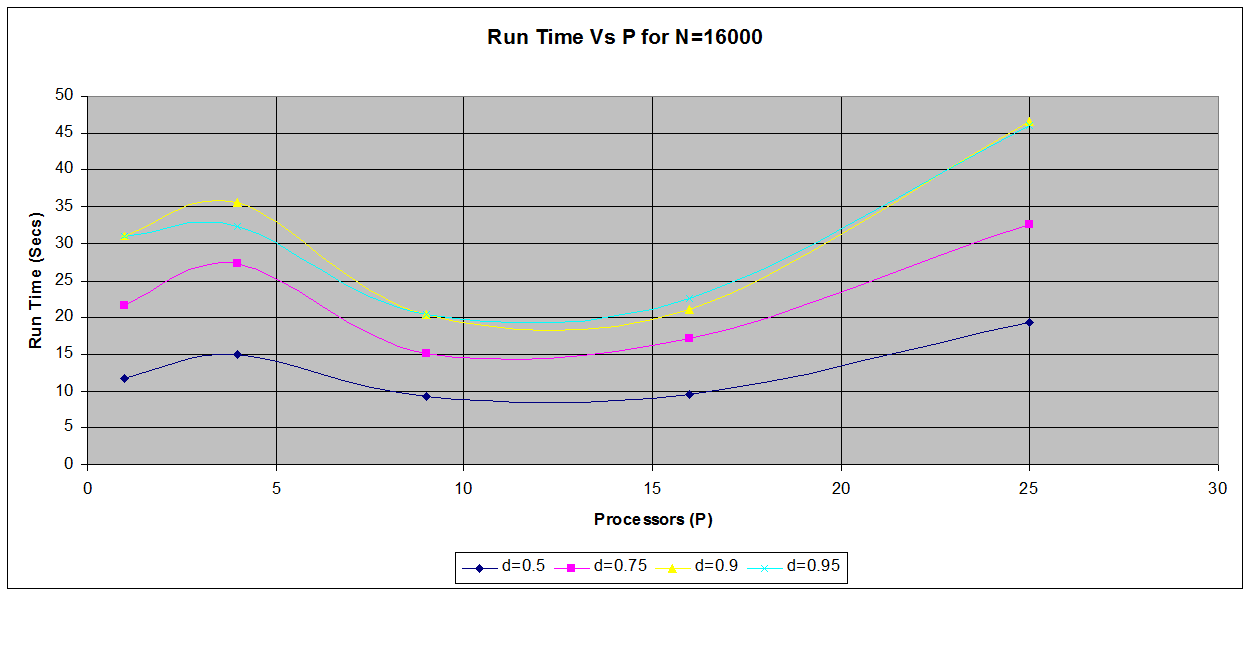
\includegraphics[scale=.46]{charts/runtime_p_d_n_16000} 
\caption{Run Time Vs P for N=16000}
\label{Run Time Vs P for N=16000}
\end{figure}

\begin{figure}[!htbp]
\centering
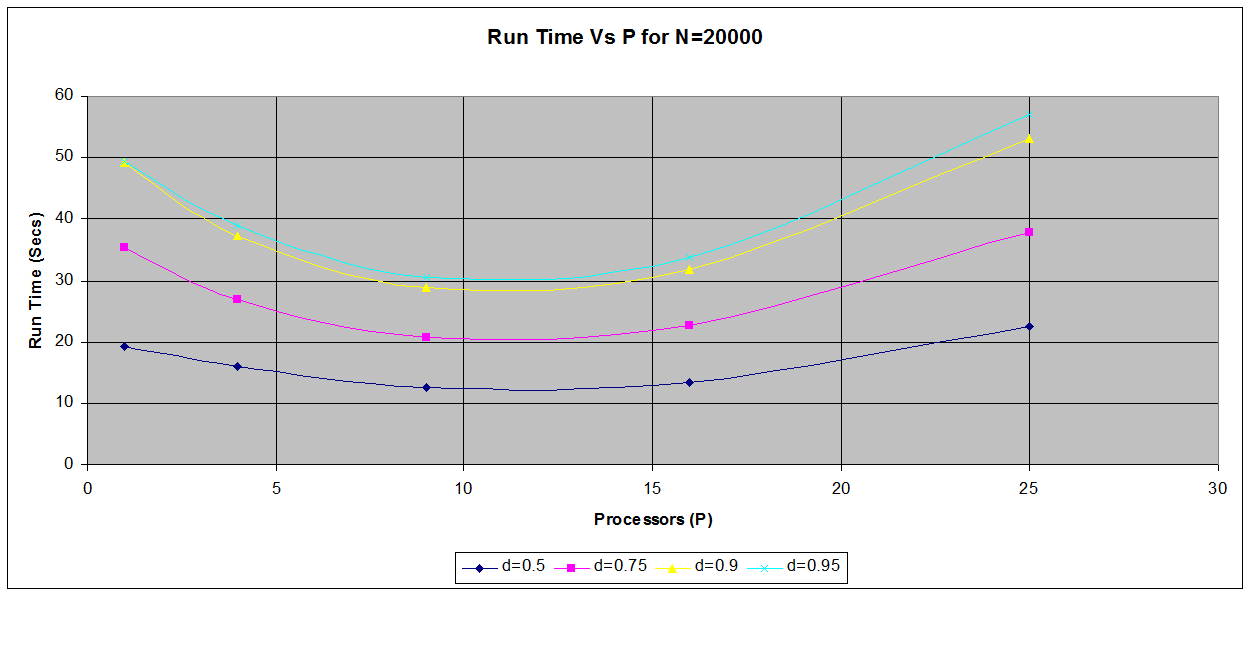
\includegraphics[scale=.46]{charts/runtime_p_d_n_20000} 
\caption{Run Time Vs P for N=20000}
\label{Run Time Vs P for N=20000}
\end{figure}

\begin{figure}[!htbp]
\centering
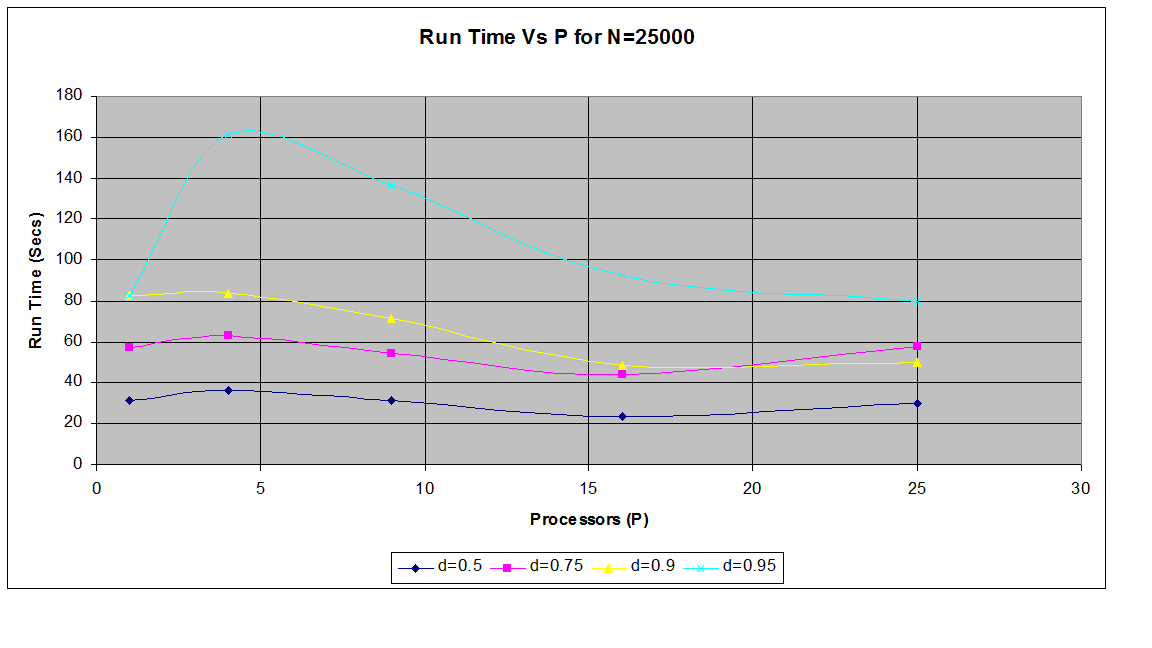
\includegraphics[scale=.46]{charts/runtime_p_d_n_25000} 
\caption{Run Time Vs P for N=25000}
\label{Run Time Vs P for N=25000}
\end{figure}


\pagebreak
\subsubsection{Runtime Performance - Plot of Run Time Vs Number of Processors P for different N for fixed Difficulty d}
The following is the performance plot of Run Time Vs Number of Processors P for different N for fixed Difficulty d

\begin{enumerate}
\item
d=0.5 $\eqref{Run Time Vs P for d=0.50}$
\item
d=0.75 $\eqref{Run Time Vs P for d=0.75}$
\item
d=0.9 $\eqref{Run Time Vs P for d=0.90}$
\item
d=0.95 $\eqref{Run Time Vs P for d=0.95}$
\end{enumerate}

\begin{figure}[!htbp]
\centering
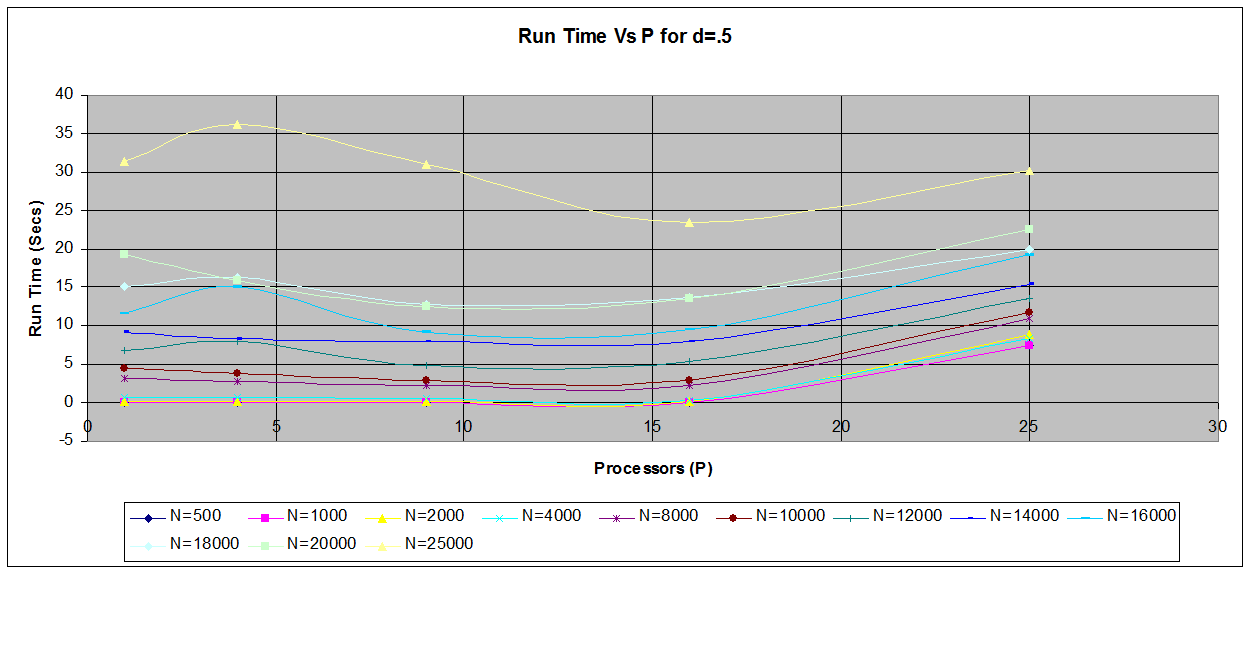
\includegraphics[scale=.46]{charts/runtime_p_n_d_50} 
\caption{Run Time Vs P for d=0.50}
\label{Run Time Vs P for d=0.50}
\end{figure}

\begin{figure}[!htbp]
\centering
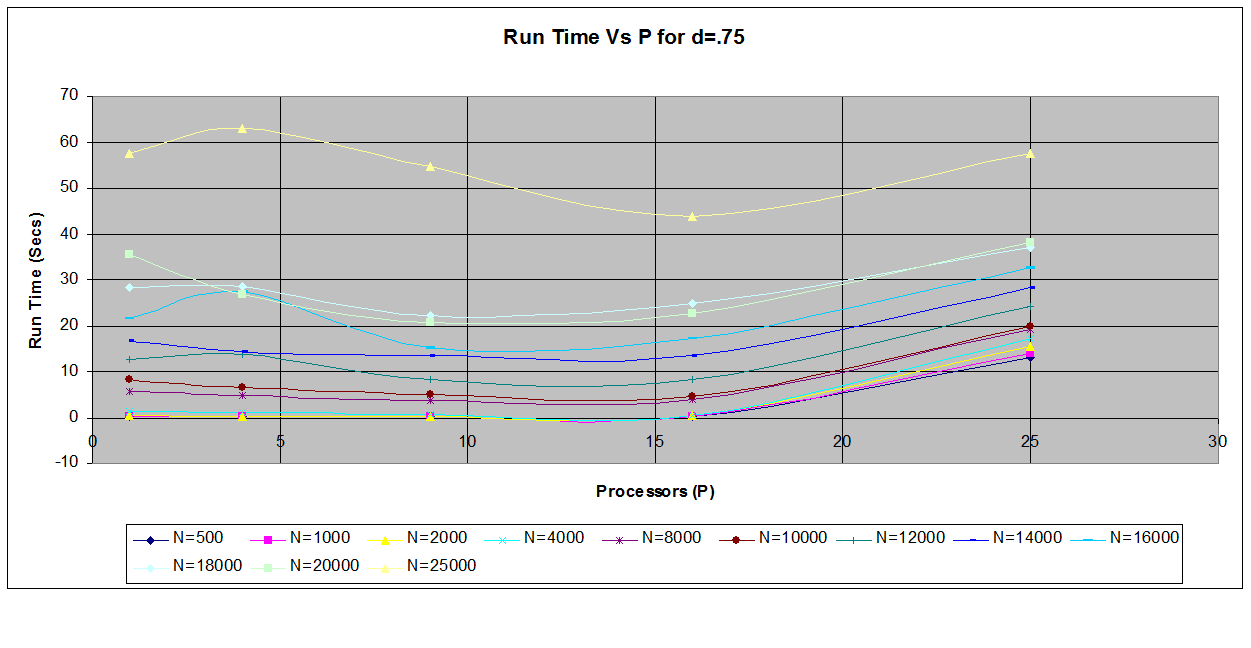
\includegraphics[scale=.46]{charts/runtime_p_n_d_75} 
\caption{Run Time Vs P for d=0.75}
\label{Run Time Vs P for d=0.75}
\end{figure}

\begin{figure}[!htbp]
\centering
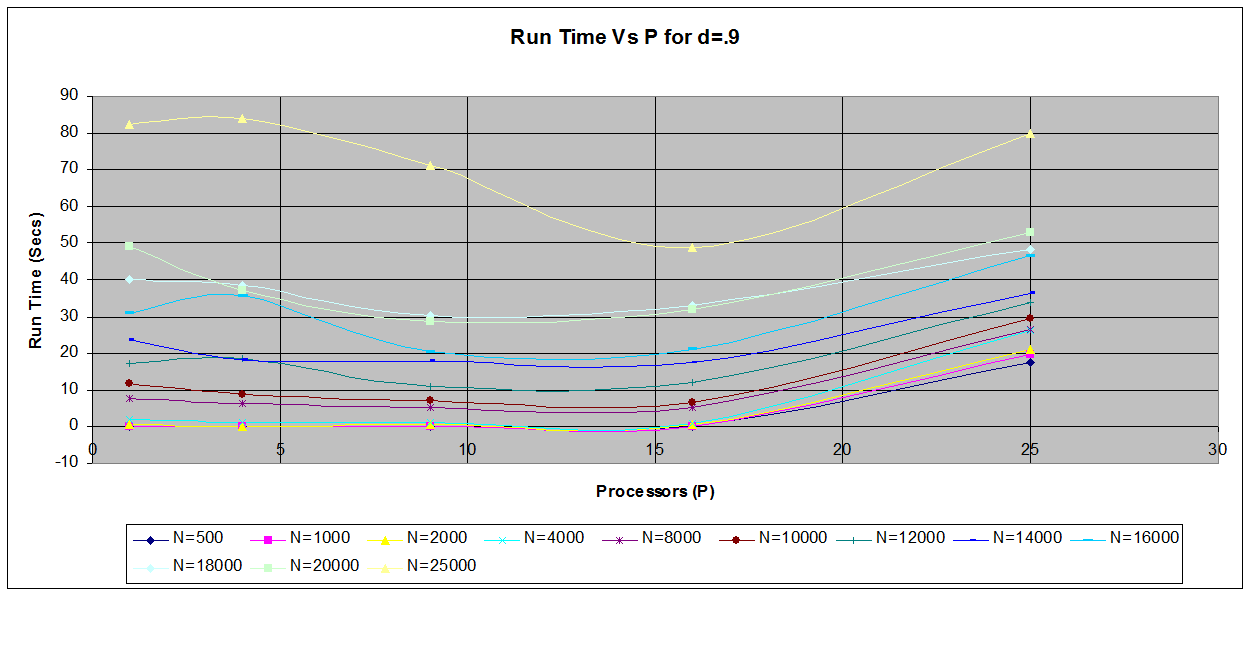
\includegraphics[scale=.46]{charts/runtime_p_n_d_90} 
\caption{Run Time Vs P for d=0.90}
\label{Run Time Vs P for d=0.90}
\end{figure}

\begin{figure}[!htbp]
\centering
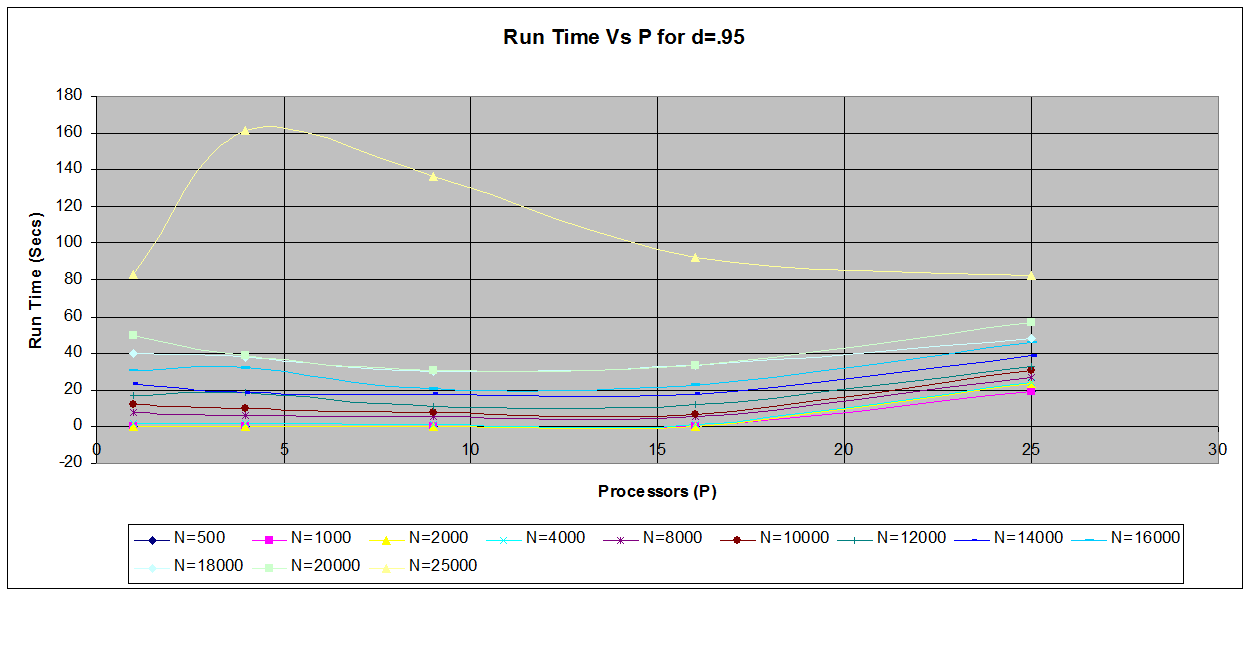
\includegraphics[scale=.46]{charts/runtime_p_n_d_95} 
\caption{Run Time Vs P for d=0.95}
\label{Run Time Vs P for d=0.95}
\end{figure}




\subsection{SpeedUp Plots}

The following are the SpeedUp Ratio plots

\pagebreak
\subsubsection{SpeedUp - Plot of SpeedUp Vs N for different levels of difficulty for fixed No of Processors P}
The following is the performance plot of SpeedUp Vs N the matrix dimension for different levels of difficulty for a fixed number of processors.

\begin{enumerate}
\item
P=4 $\eqref{SpeedUp Vs N for P=4}$
\item
P=9 $\eqref{SpeedUp Vs N for P=9}$
\item
P=16 $\eqref{SpeedUp Vs N for P=16}$
\item
P=25 $\eqref{SpeedUp Vs N for P==25}$
\end{enumerate}

\begin{figure}[!htbp]
\centering
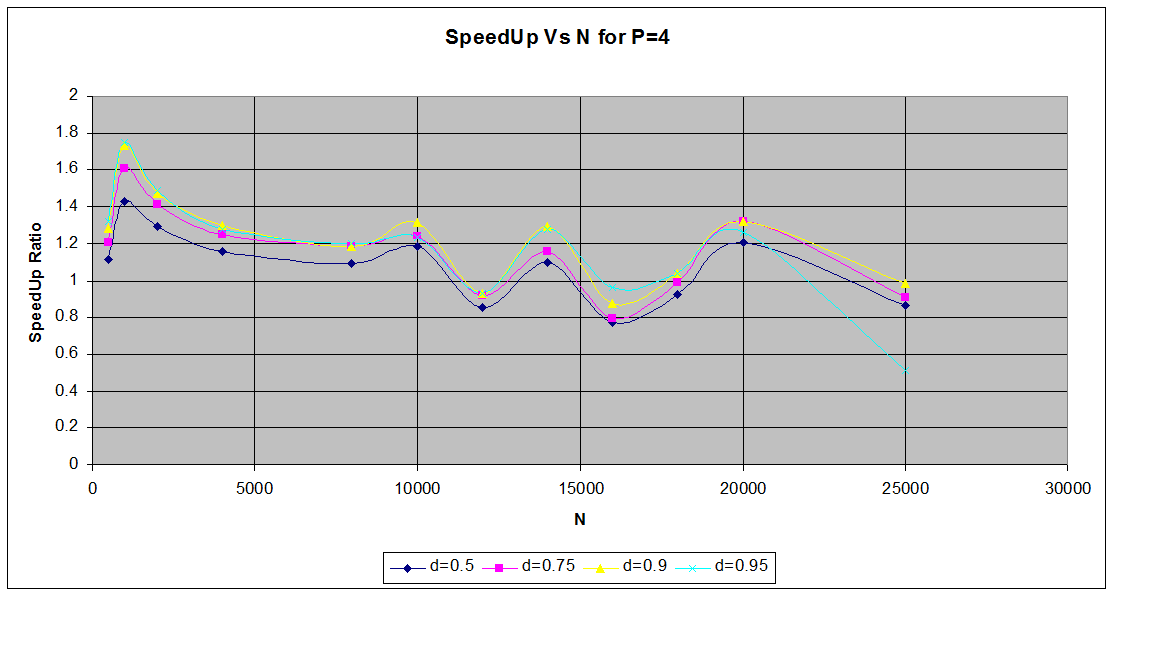
\includegraphics[scale=.46]{charts/speedup_n_d_p_4} 
\caption{SpeedUp Vs N for P=4}
\label{SpeedUp Vs N for P=4}
\end{figure}

\begin{figure}[!htbp]
\centering
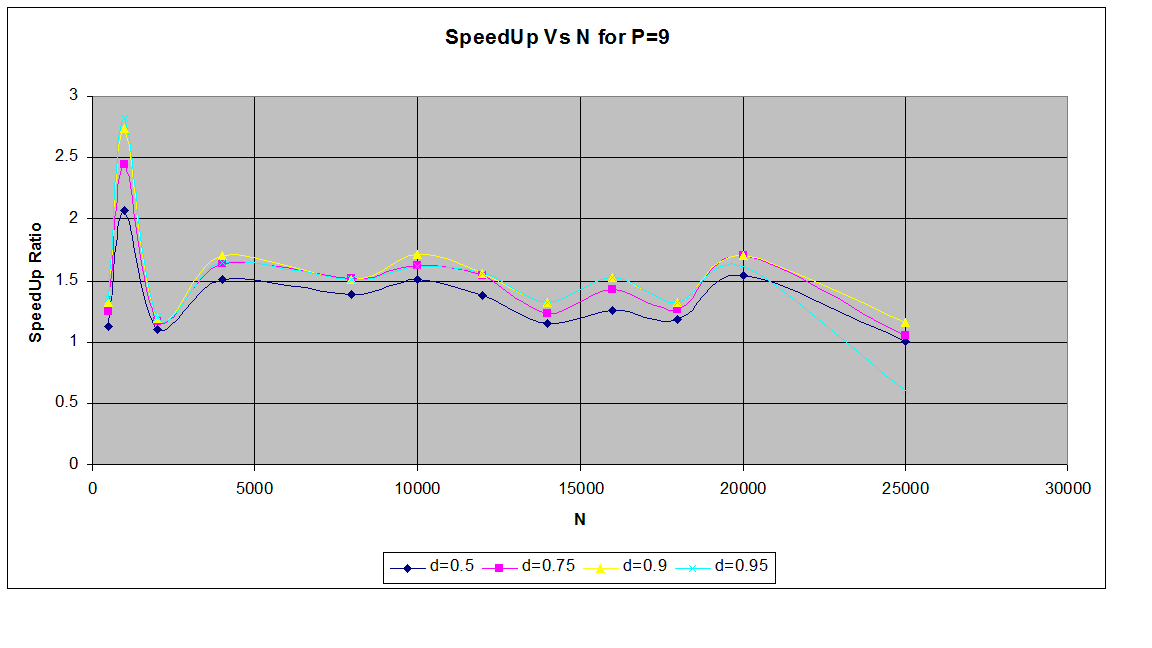
\includegraphics[scale=.46]{charts/speedup_n_d_p_9} 
\caption{SpeedUp Vs N for P=9}
\label{SpeedUp Vs N for P=9}
\end{figure}

\begin{figure}[!htbp]
\centering
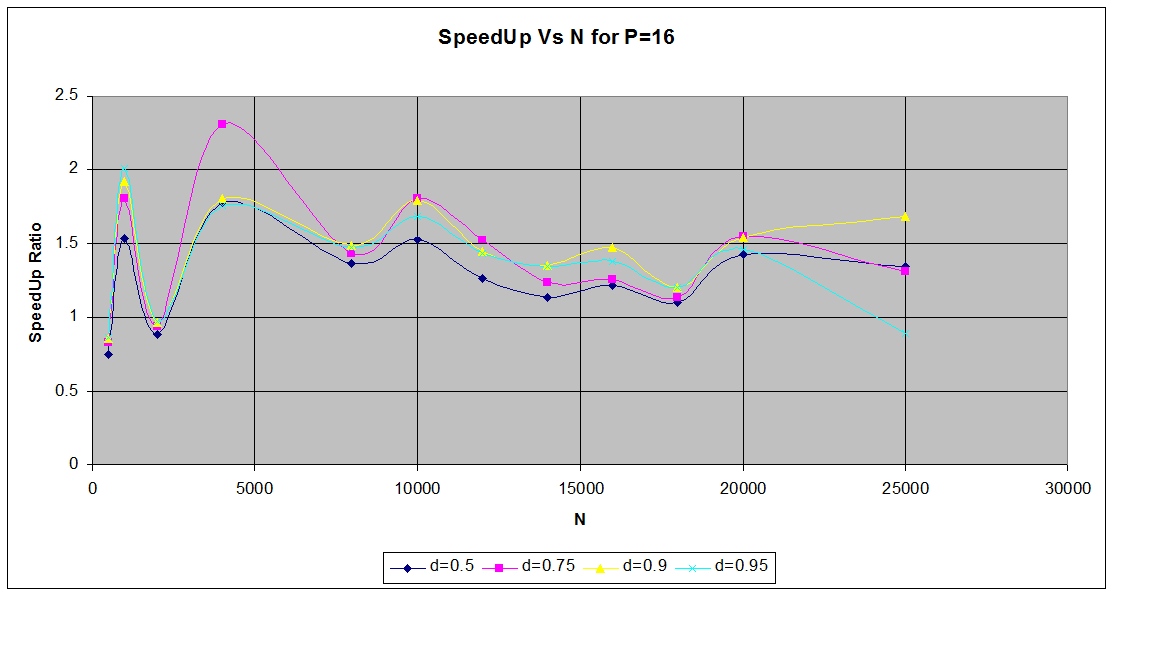
\includegraphics[scale=.46]{charts/speedup_n_d_p_16} 
\caption{SpeedUp Vs N for P=16}
\label{SpeedUp Vs N for P=16}
\end{figure}

\begin{figure}[!htbp]
\centering
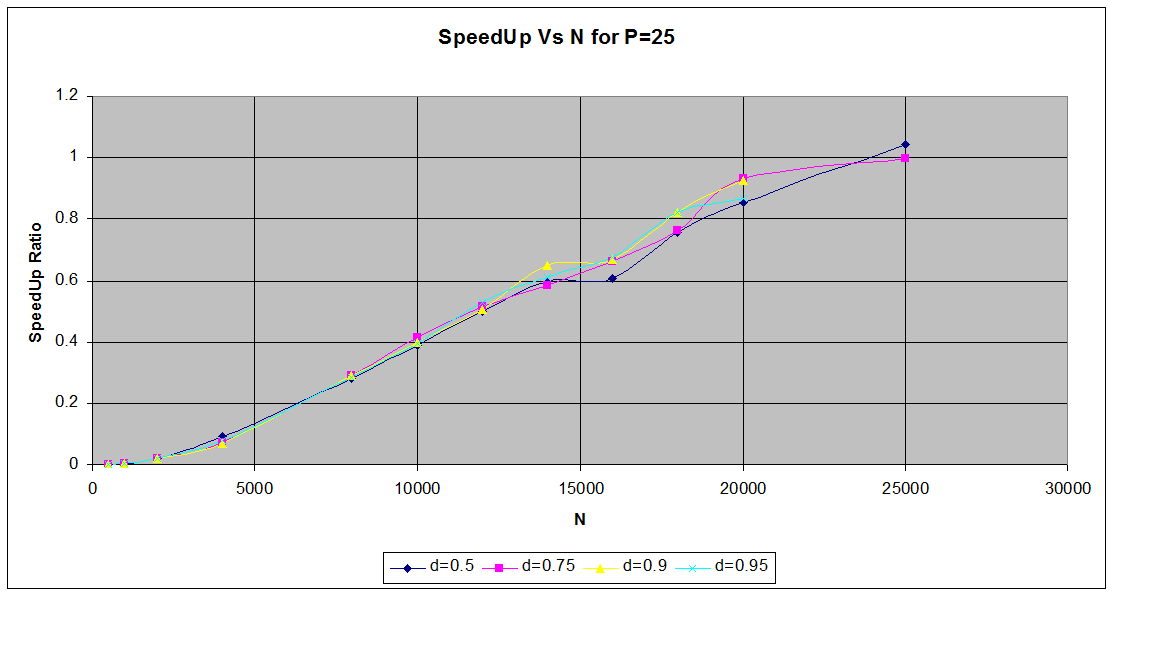
\includegraphics[scale=.46]{charts/speedup_n_d_p_25} 
\caption{SpeedUp Vs N for P==25}
\label{SpeedUp Vs N for P==25}
\end{figure}



\pagebreak
\subsubsection{Runtime Performance - Plot of SpeedUp Vs Number of Processors P for different levels of difficulty for fixed size N}
The following is the performance plot of SpeedUp Vs Number of Processors P for different levels of difficulty for fixed matrix size N

\begin{enumerate}
\item
N=1000 $\eqref{SpeedUp Vs P for N=1000}$
\item
N=8000 $\eqref{SpeedUp Vs P for N=8000}$
\item
N=16000 $\eqref{SpeedUp Vs P for N=16000}$
\item
N=20000 $\eqref{SpeedUp Vs P for N=20000}$
\item
N=25000 $\eqref{SpeedUp Vs P for N=25000}$
\end{enumerate}

\begin{figure}[!htbp]
\centering
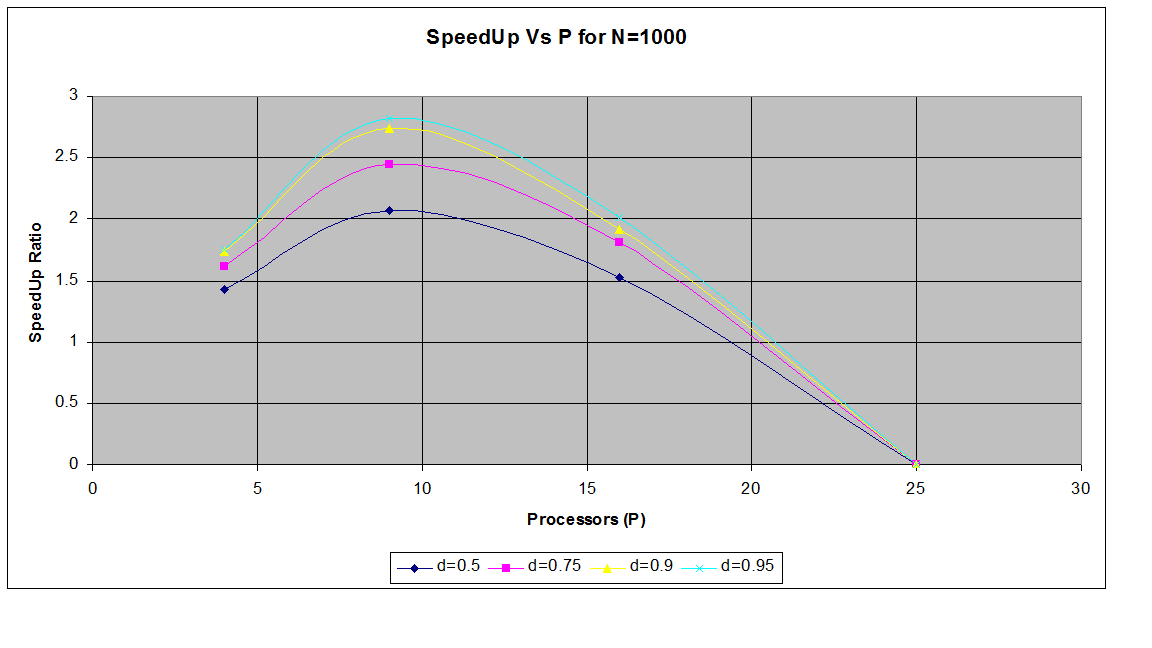
\includegraphics[scale=.46]{charts/speedup_p_d_n_1000} 
\caption{SpeedUp Vs P for N=1000}
\label{SpeedUp Vs P for N=1000}
\end{figure}

\begin{figure}[!htbp]
\centering
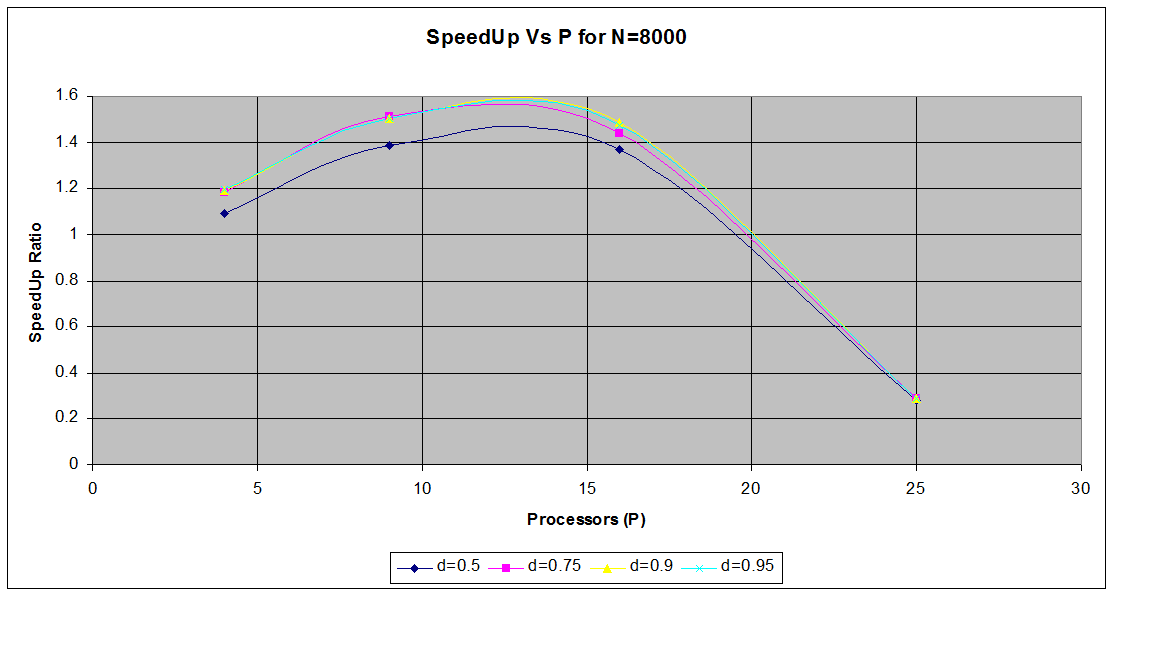
\includegraphics[scale=.46]{charts/speedup_p_d_n_8000} 
\caption{SpeedUp Vs P for N=8000}
\label{SpeedUp Vs P for N=8000}
\end{figure}

\begin{figure}[!htbp]
\centering
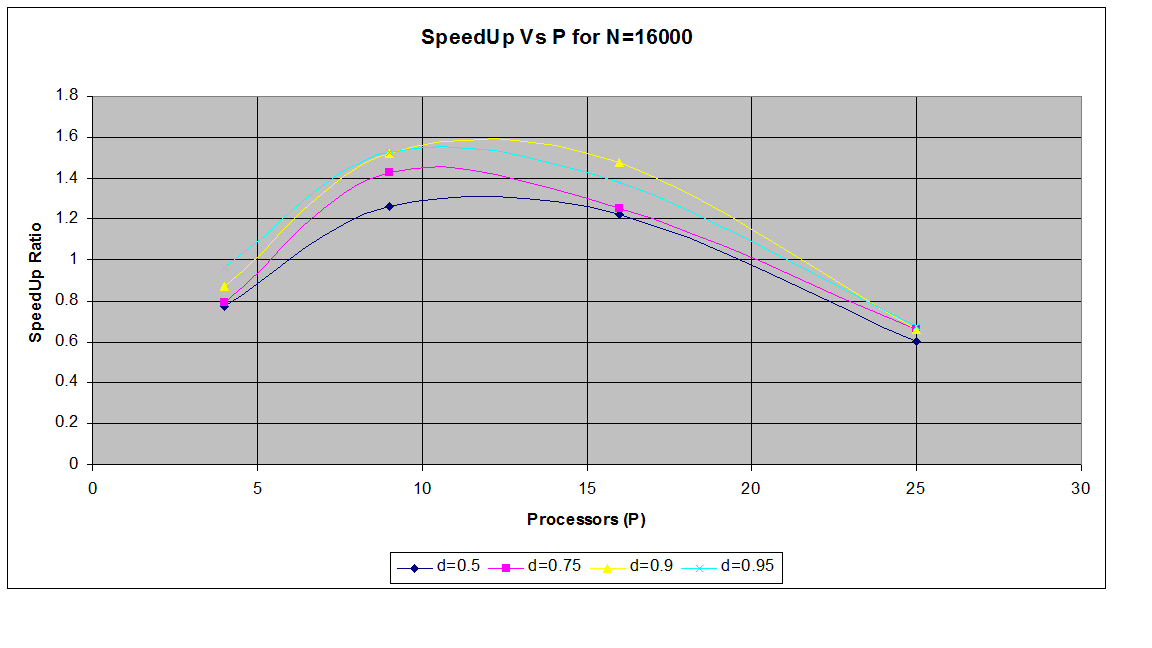
\includegraphics[scale=.46]{charts/speedup_p_d_n_16000} 
\caption{SpeedUp Vs P for N=16000}
\label{SpeedUp Vs P for N=16000}
\end{figure}

\begin{figure}[!htbp]
\centering
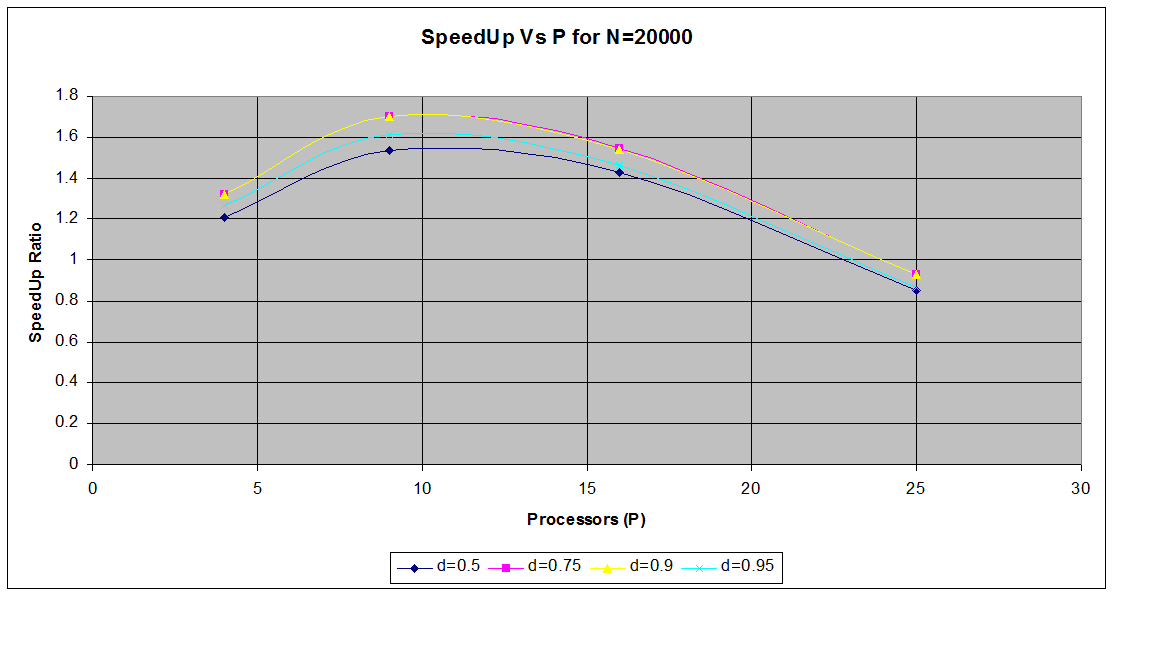
\includegraphics[scale=.46]{charts/speedup_p_d_n_20000} 
\caption{SpeedUp Vs P for N=20000}
\label{SpeedUp Vs P for N=20000}
\end{figure}

\begin{figure}[!htbp]
\centering
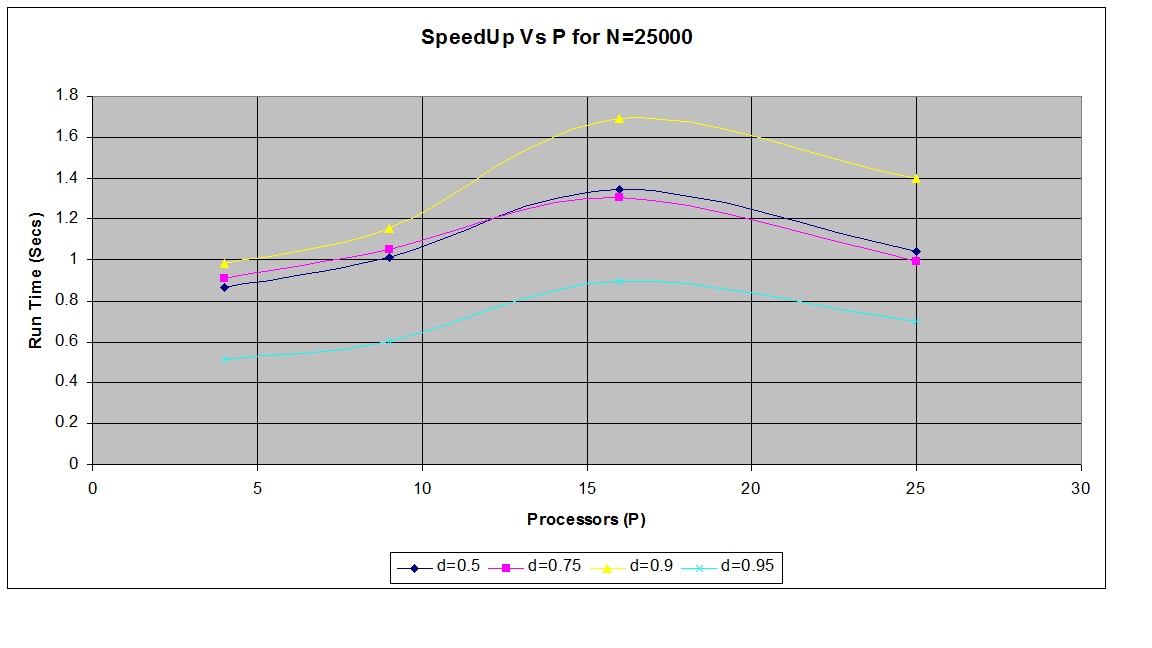
\includegraphics[scale=.46]{charts/speedup_p_d_n_25000} 
\caption{SpeedUp Vs P for N=25000}
\label{SpeedUp Vs P for N=25000}
\end{figure}


\pagebreak
\subsubsection{Runtime Performance - Plot of SpeedUp Vs Number of Processors P for different N for fixed Difficulty d}
The following is the performance plot of SpeedUp Vs Number of Processors P for different N for fixed Difficulty d

\begin{enumerate}
\item
d=0.5 $\eqref{SpeedUp Vs P for d=0.50}$
\item
d=0.75 $\eqref{SpeedUp Vs P for d=0.75}$
\item
d=0.9 $\eqref{SpeedUp Vs P for d=0.90}$
\item
d=0.95 $\eqref{SpeedUp Vs P for d=0.95}$
\end{enumerate}

\begin{figure}[!htbp]
\centering
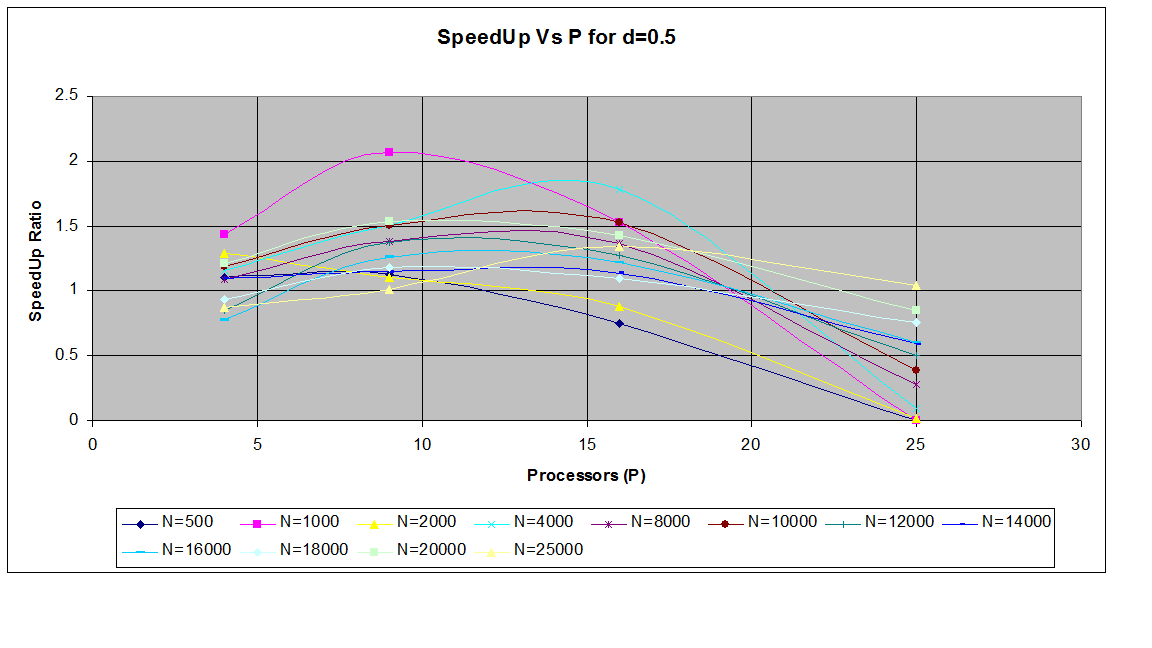
\includegraphics[scale=.46]{charts/speedup_p_n_d_50} 
\caption{SpeedUp Vs P for d=0.50}
\label{SpeedUp Vs P for d=0.50}
\end{figure}

\begin{figure}[!htbp]
\centering
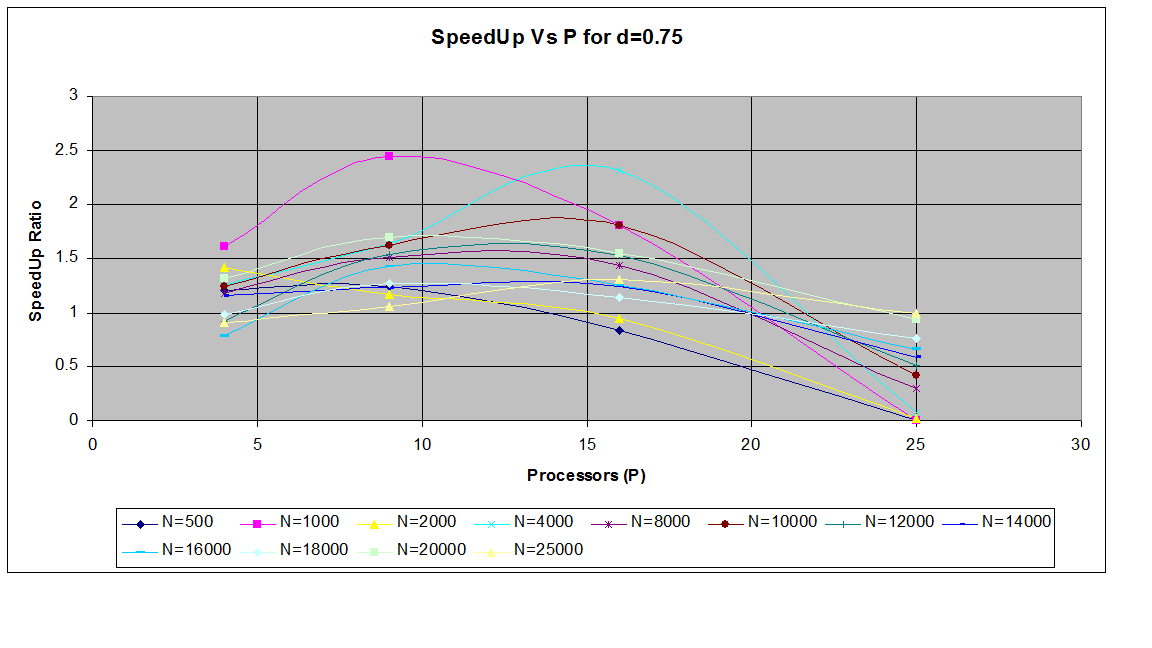
\includegraphics[scale=.46]{charts/speedup_p_n_d_75} 
\caption{SpeedUp Vs P for d=0.75}
\label{SpeedUp Vs P for d=0.75}
\end{figure}

\begin{figure}[!htbp]
\centering
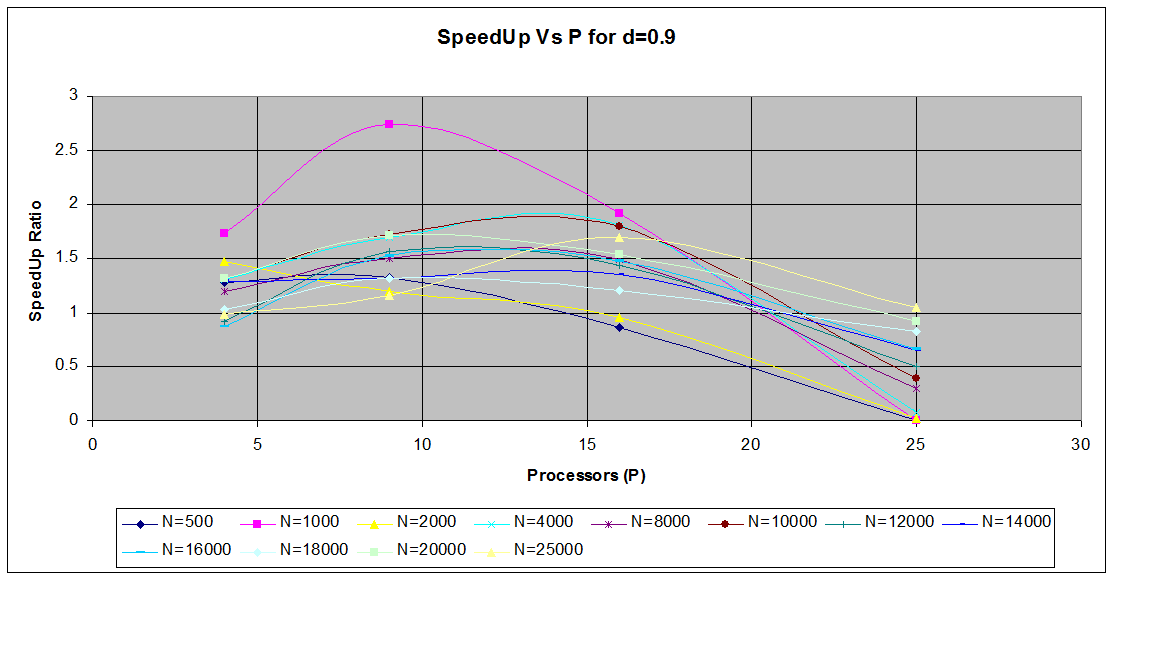
\includegraphics[scale=.46]{charts/speedup_p_n_d_90} 
\caption{SpeedUp Vs P for d=0.90}
\label{SpeedUp Vs P for d=0.90}
\end{figure}

\begin{figure}[!htbp]
\centering
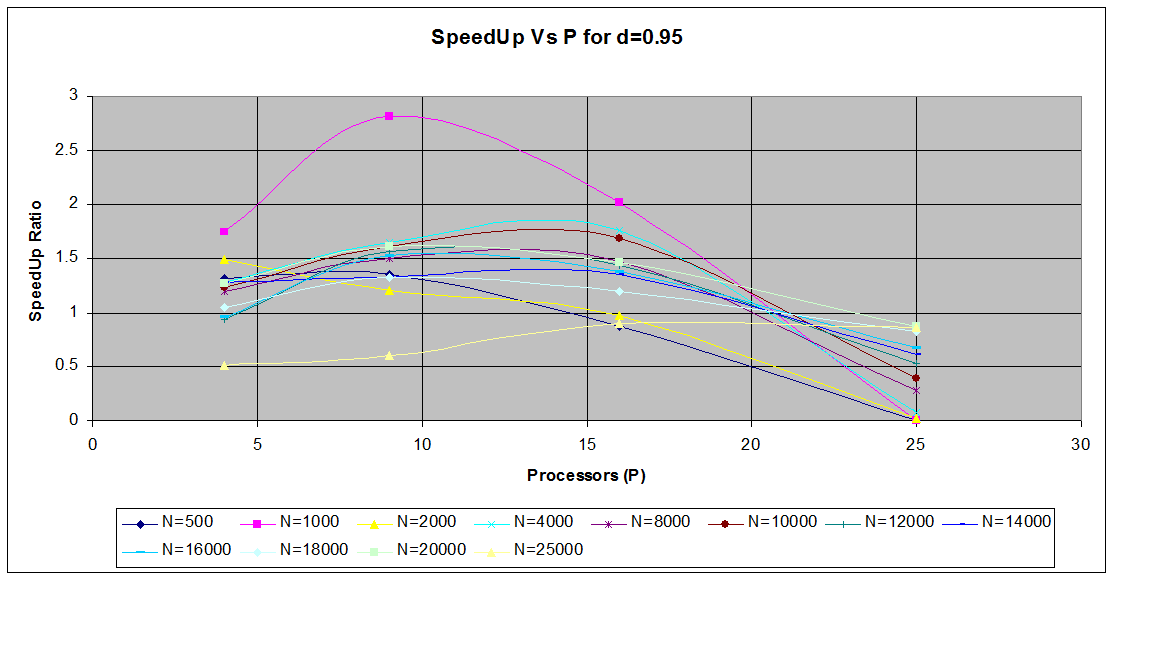
\includegraphics[scale=.46]{charts/speedup_p_n_d_95} 
\caption{SpeedUp Vs P for d=0.95}
\label{SpeedUp Vs P for d=0.95}
\end{figure}



\pagebreak
\section{Conclusions}
\begin{itemize}
\item
The serial runtime of the algorithm is of the order of
\begin{align}
T(n,1) &= iterations * \mathcal{O}(n^2)\label{p1_runtime_1}
\end{align}
\item
The parallel algorithm has a complexity of
\begin{align}
T(n,p) &= iterations*[\mathcal{O}(\frac{n^2}{p})] + iterations*[\mathcal{O}(\tau \log \sqrt{p} + \mu \frac{n}{\sqrt{p}})] + \mathcal{O}(\tau \log \sqrt{p} + \mu n^2) \label{p1_runtime_2}
\end{align}
\item
At very small values of $n$, the communication overhead given by $iterations*[\mathcal{O}(\tau \log \sqrt{p} + \mu \frac{n}{\sqrt{p}})] + \mathcal{O}(\tau \log \sqrt{p} + \mu n^2)$, especially $\tau \log \sqrt{p}$ would dominate over computation costs. So at very low values of $n$ it might make no sense to try to parallel algorithm as it has no speed up over the serial algorithm. This is borne out by the graphs at values of $n<1000$
\item
For the Serial algorithm the run time increases with $N$ and is higher for higher difficulty levels 
\item
For the Parallel algorithm for a given number of fixed processors, the run time
\begin{enumerate}
\item
Increases as $N$ is increased
\item
Is higher with increased difficulty
\item
Increases at a higher rate at higher values on $N$
\end{enumerate}
\item
For the Parallel algorithm if $N$ is fixed then
\begin{enumerate}
\item
Initially for low values of $p$, the SpeedUp increases as we increase the number of processors $p$
\item
We have a point of inflexion in the curve where run time is lowest at a certain value of $P$ and then increases again as P is increased. This indicates that for a given problem size of $N$ there is a optimum number of processors $P$ which give the best run time. The optimum value of $P$ for a fixed problem size of $N$ is the value at which the computation cost of the parallel algorithm $iterations*[\mathcal{O}(\frac{n^2}{p})]$ still dominates over the communication cost $iterations*[\mathcal{O}(\tau \log \sqrt{p} + \mu \frac{n}{\sqrt{p}})] + \mathcal{O}(\tau \log \sqrt{p} + \mu n^2)$  
\item
It can also seen that the value of the point of inflexion , ie $P$ the number of processors at which runtime is the least, gets higher as the fixed value of $N$ is increased. This indicates that as $N$ is increased the computation cost of the parallel algorithm $iterations*[\mathcal{O}(\frac{n^2}{p})]$ is higher and thus can absorb the larger communication cost $iterations*[\mathcal{O}(\tau \log \sqrt{p} + \mu \frac{n}{\sqrt{p}})] + \mathcal{O}(\tau \log \sqrt{p} + \mu n^2)$ of a larger $N$
\end{enumerate}
\item
Higher the difficulty level higher is the run time. The spread of the run time is higher at higher values of $N$
\item
As seen with Run Time, SpeedUp is also fairly stable in a small range but falls off gradually as either $N$ decreases below a threshold or is increased beyond a threshold for a fixed number of processors
\begin{enumerate}
\item
SpeedUp decreases as $N$ is increased beyond a certain threshold for a given fixed number of processors, showing that for a given fixed number of processors as $N$ is increased communication ( specifically the brandwidth overhead in  $iterations*[\mathcal{O}(\tau \log \sqrt{p} + \mu \frac{n}{\sqrt{p}})] + \mathcal{O}(\tau \log \sqrt{p} + \mu n^2)$) begins to dominate over computation cost for the Parallel Algorithm.
\end{enumerate}
\item
It can be seen from the graph that SpeedUp $<1$ for values of $N < 1000 $. This is again as expected as communication costs of the parallel algorithm will dominate over computation costs at low values of $N$
\item
Thus we can conclude that
\begin{enumerate}
\item
At low values of $N$, parallel algorithm does not have a utility because of communication overheads
\item
For a given fixed value of $N$, SpeedUp of the parallel algorithm increases initially as $P$ is increased from a low value of $P$. However on reaching a optimum value of SpeedUp for a certain value of $P$, the SpeedUp then begins to fall gradually as $P$ is increased further
\item
So for a given problem size of $N$ there is a optimum value of $P$ to get the best SpeedUp
\end{enumerate}
\end{itemize}


% Generate the bibliography.
\bibliography{latex-sample}
\bibliographystyle{unsrt}

\end{document}